\documentclass[11pt]{article}		% set type of document and font size
\usepackage[margin=1in]{geometry}	% set all margins to one inch
\usepackage[utf8]{inputenc}			% basic formatting package
\usepackage[english]{babel}			% specify language explicitly
\usepackage{amsmath}				% more sophisticated math typesetting
\usepackage[square,numbers]{natbib}	% bibliography management
\bibliographystyle{apsrev4-2}		% bibliography style
\usepackage{graphicx,caption}		% for figures

\usepackage{hyperref}
% set up hyperlinking
\hypersetup{
	colorlinks=true,
	linkcolor=blue,
	filecolor=blue,      
	urlcolor=blue,
}

% options for \maketitle
\title{LaTex Template}
\author{Grant Gorman}
\date{\today}

\begin{document}

\maketitle

\setlength{\parindent}{0in} % remove autoindentation
\setlength{\parskip}{\baselineskip} % space out paragraphs

\begin{abstract}
	
	This document describes how to install, configure, and use LaTex with the TexMaker editor and TexLive distribution. 

\end{abstract}

\section{Installing and Configuring LaTex} 
\label{sec:install}
In order to use LaTex you will need a LaTex editor and a Tex distribution. I  recommend using  TexMaker (\href{https://www.xm1math.net/texmaker/index.html}{link}) or TexStudio (\href{https://www.texstudio.org/}{link}) and TexLive (\href{https://www.tug.org/texlive/acquire-netinstall.html}{link}, click on $<$install-tl-windows.exe$>$). Once you have installed an editor and distribution, add the TexLive distribution to you system search path. The default distribution path is typically $<$C$:\backslash $texlive$\backslash 2021\backslash$bin$\backslash$win32$>$ on a Windows computer. 

The TexMaker compiler will need to be configured. There are two commands you'll need to use: $<$PDFLaTeX$>$, $<$BibTex$>$, and $<$View PDF$>$. For a new document, the PDF command must be run first to create a .aux file. All of your references will be contained within a .bib file, and the BibTex command must be run each time changes are made to this file. This command creates a $<$.bbl$>$ file that is linked to the .aux file, which allows your document to see the reference identifiers. Strangely, in order for the reference numbers to be linked properly, you need to run the PDFLaTeX command twice whenever the .bbl file is updated. This is a bit of a pain, but you can configure the Quick Build tool, accessed with F1 and configured at $<$options$\rightarrow$Configure Texmaker$>$
, to run PDFLaTeX, BibTex, PDFLaTeX$\times2$, view PDF. This makes the compiling process a bit slower, so I tend to leave the Quick Build tool as default (i.e., run PDFLaTeX and View PDF). I just remember that I have to recompile the .bbl when I update the .bib because the default Quick Build tool is really fast.

TexStudio won't need any extra compiling, so I recommend using that.


\section{Setting Up Document}
\label{sec:setup}
The default name for the main Tex document is $<$ms.tex$>$, as is the case with this template. When submitting manuscripts to journals, they will want the files named this way. As discussed in Sec. \ref{sec:install}, press F6 to create the .aux file, then you can compile the .bib into .bbl as needed. As you update ms.tex, using the default Quick Build to run PDFLaTeX and View PDF will be the quickest way to update the PDF.

\section{Using BibTex for References}
\label{sec:bib}

I like to use natbib as my reference compiler and the APS bibliography style (both defined above). Here is an example for how to cite an article \cite{gwb2021}. Note that this reference identifier, gwb2021, is Tom's preferred format for reference identifiers. The first three letters are the first letter of the last name of the first three authors on a paper and then the published date. As I noted in Sec. \ref{sec:install}, you need to run the BibTex to update the .bbl file to be consistent with the updated .bib. The .bib file I use here, $<$UltracoldNeutralPlasmas.bib$>$, was created using Zotero. Zotero allows you to export the contents of a given folder - or the entire library - into a .bib file for use with BibTex. This .bib file only includes my ultracold neutrla plasma papers, but I typically export my entire library, which contains all the references I've ever used in a paper. This way I won't have to update the .bib file too much as I write, and by extension won't have to run the BibTex command much. For this reason I typically leave the Quick Build command as default.

\section{Figures and Labels}
\label{sec:figs}

Here is how to create and reference a figure Fig. \ref{fig:exp-schem}, same as referring to any other label. Note that most journals want figure files submitted in .eps format. This is generally because they can open and edit .eps figure files after submission to adjust colors and the like without sending back to the authors. You can use .png and .jpeg, but prefer .eps to be used to it. Equations can be referred to as well. Here is the equation for the Coulomb coupling parameter (Eq. \ref{eq:gamma}):
\begin{equation}
\label{eq:gamma}
\Gamma=\frac{e^2}{4\pi\epsilon_0 a_{ws} k_B T}
\end{equation}
where $a_{ws}=(3/4\pi n)^{1/3}$ is an example of how to include in-line math.

\begin{figure}[h]
	
	\centering
	\captionsetup{width=.8\linewidth} % make caption textwidth same as graphic width
	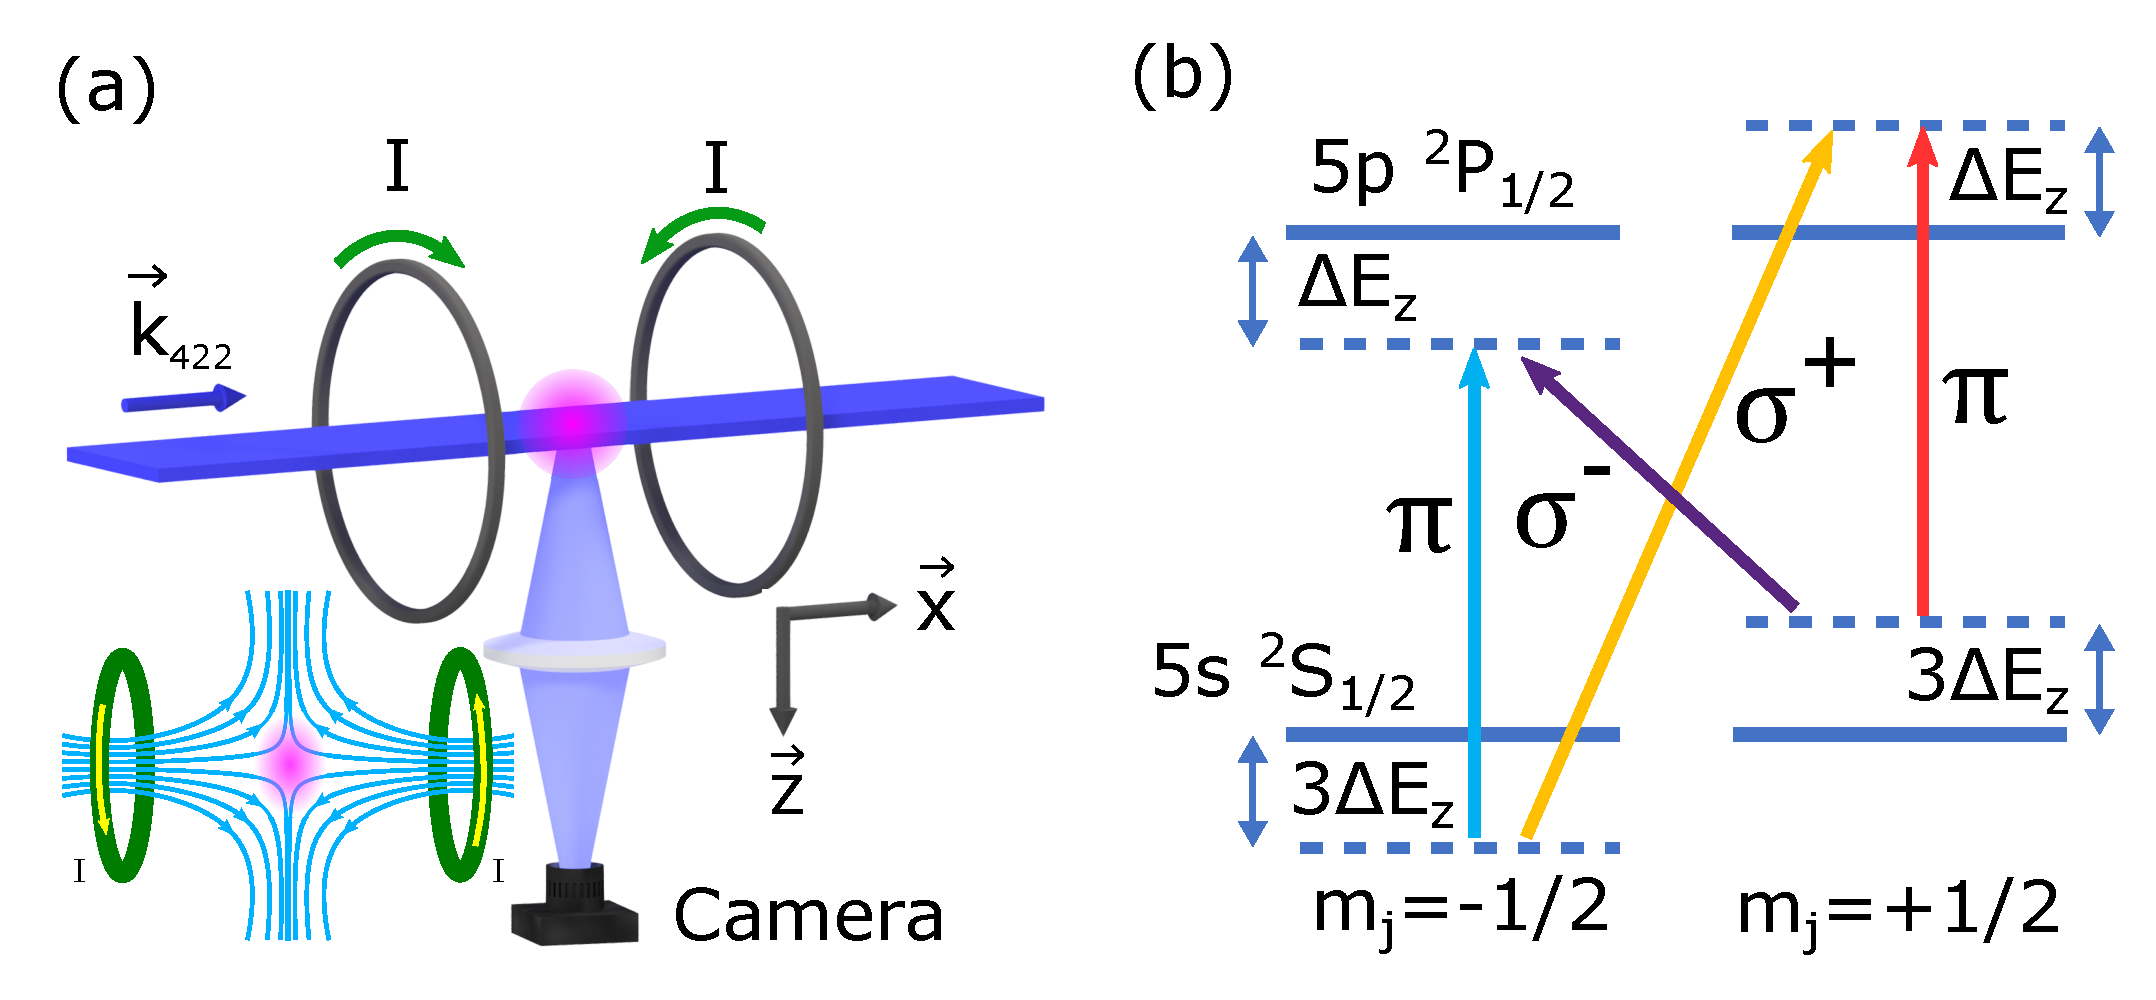
\includegraphics[width=0.75\textwidth]{schematic-with-levels}
	\caption{(a) Experimental schematic for laser-induced fluorescence imaging LIF) and application of quadrupole magnetic fields using anti-Helmholtz coils (inset depicts field lines). The plasma is illuminated by a thin sheet of 422-nm light that propagates along the x axis and is linearly polarized along the y axis. The ion fluorescence is imaged onto an intensified CCD camera using a 1:1 optical relay along the z axis. (b) Sr levels coupled by LIF laser with (dashed) and without (solid) Zeeman shifts.}
	\label{fig:exp-schem}
\end{figure}

\section{Overleaf - Online LaTeX Editor}

\href{https://www.overleaf.com/}{Overleaf} is a free Online LaTeX editor that uses the TexLive distribution. The attraction to Overleaf is its ease of use (no installation required) and it makes collaborating easy. Unfortunately, the free Overleaf version only allows you to share with one collaborator and does not allow for version control via Git. You can link share, but that is much less secure as anyone who gets the link can edit the document. Another issue with Overleaf is that it compiles figures with low resolution. I often find small text in my figures looks blurry, but when compiled locally with TexMaker the figures look great. 

Tom tends to like collaborating via Overleaf, so that is what I default to when I am writing a paper. I just make sure to download the source files every so often as a backup. For all other endeavors, I prefer using TexMaker locally so that I can have my files backed up either via Git or Google Drive. You will also find as projects get large that compiling locally will be faster. Whatever you choose to do, just make sure you are backing up your files somehow.

\bibliography{UltracoldNeutralPlasmas.bib} 

\end{document}




